\documentclass{article}
\usepackage[utf8]{inputenc}

\usepackage{listings}
\usepackage{algorithm}
\usepackage{algorithmic}
\usepackage{color}
\usepackage{graphicx} %package to manage images

%New colors defined below
\definecolor{codegreen}{rgb}{0,0.6,0}
\definecolor{codegray}{rgb}{0.5,0.5,0.5}
\definecolor{codepurple}{rgb}{0.58,0,0.82}
\definecolor{backcolour}{rgb}{0.95,0.95,0.92}

%Code listing style named "mystyle"
\lstdefinestyle{mystyle}{
  backgroundcolor=\color{backcolour},   commentstyle=\color{codegreen},
  keywordstyle=\color{magenta},
  numberstyle=\tiny\color{codegray},
  stringstyle=\color{codepurple},
  basicstyle=\footnotesize,
  breakatwhitespace=false,         
  breaklines=false,                 
  captionpos=b,                    
  keepspaces=true,                 
  numbers=left,                    
  numbersep=5pt,                  
  showspaces=false,                
  showstringspaces=false,
  showtabs=false,                  
  tabsize=2
}

%"mystyle" code listing set
\lstset{style=mystyle}

\begin{document}
\centerline{\sc \large EECE 7360 Project 4}
\vspace{.5pc}
\centerline{\sc Garrett Goode and Daniel Hullihen}
\centerline{\it Spring 2017}

\section{Introduction}
The subset sum problem (also referred to as the ``exact knapsack problem'')
is defined below.

\textit{Let A = $\{a_1, ..., a_n\}$ represent some set of integers. Given a sum s, find a subset $A' \subset A$ such that
  $$s = \sum_{i=1}^n a_i, for 1 \le i \le n.$$}
In other words, if we are given a list of numbers and some target sum, we want
to find the numbers in the list that would add up to the target sum. Put as a decision
problem, the question would be ``Is there a subset A' of A where the sum of the
elements of A' is s?''

In this project, we examined LP and ILP techniques, and then ran our ILP model against our suite of instances.

\section{ILP Formulation}
The implementation of the ILP formulation we utilized is given by the following AMPL model pseudo-code.

\begin{algorithm}
  \caption{AMPL Model for Subset Sum}
  \label{Model}
  \begin{algorithmic}
    \STATE{$values \gets$} \COMMENT{input set}
    \STATE{$X \gets []$} \COMMENT{empty binary array}
    \STATE{}
    \ENSURE{}
    \STATE{values[i] * X[i] is maximal}
    \STATE{}
    \REQUIRE{}
    \STATE{sum(values[i] * X[i]) = target }
  \end{algorithmic}
\end{algorithm}

First parameters are created to store the input data for the problem instance, the set of integers and 
the target. A second array of binary values is created to track which members of the input set will form 
the subset that represents the solution.

We elected to maximize the sum of the subset as our objective function, so that even in a situation 
with no solution we would still be able to achieve the best possible value. This was also the way our 
greedy algorithm behaved, so it would make it easier to compare the results.

Lastly, our sole condition guaranteed that the sum of the subset would have to be equal to the target. 
This way, optimal solutions would always stop at the target, despite trying to "maximize" the sum.

\section{LP Lower Bound}
Unsurprisingly, the LP lower bounds we calculated essentially match the ILP results discussed later 
in the Results portion of the report. This holds with our expectation, as since subset sum seeks an 
exact value. One notable difference was the LP models ran much faster than their ILP counterparts, as 
evidenced by the figures below.

\begin{figure}[h]
\centering
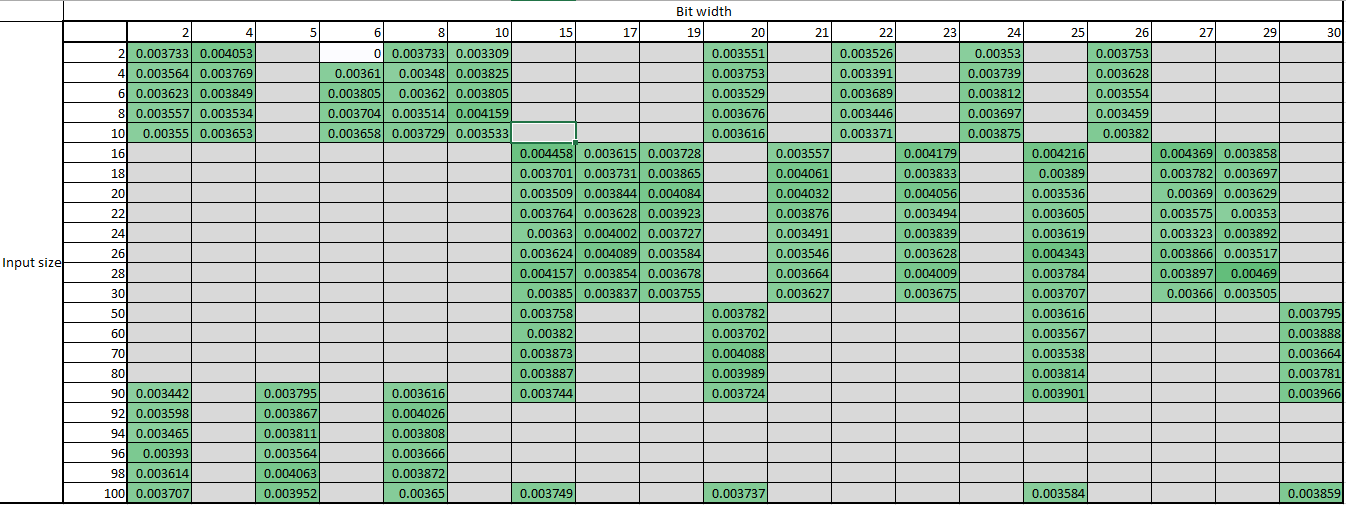
\includegraphics[width=12cm]{p4_LP_rt.png}
\caption{Runtimes for LP subset sum models}
\label{fig:lp_rt}
\end{figure}

\begin{figure}[h]
\centering
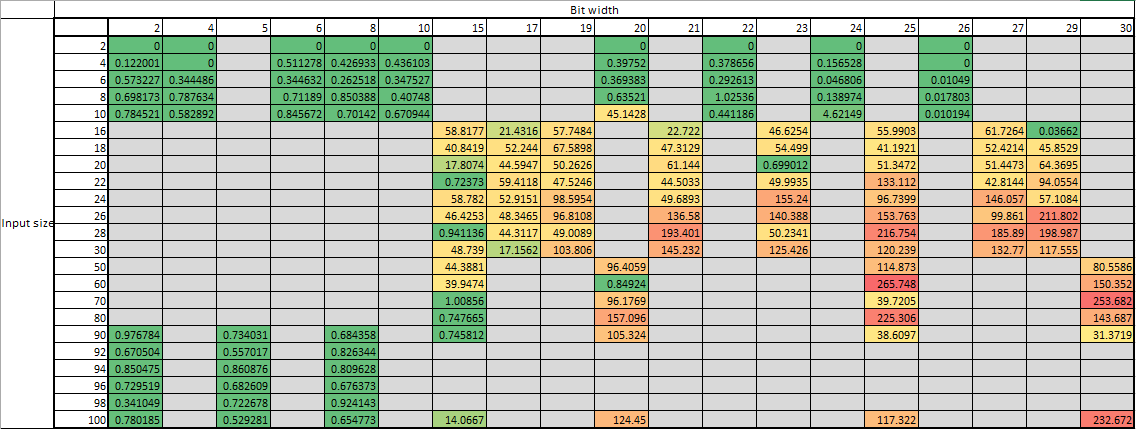
\includegraphics[width=12cm]{p4_ILP_rt.png}
\caption{Runtimes for ILP subset sum models}
\label{fig:ilp_rt}
\end{figure}

\section{Results}

The results are presented in Figure~\ref{fig:ilp} below. The vertical axis represents the
input size and the horizontal axis the word length of the elements in bits.

\begin{figure}[h]
\centering
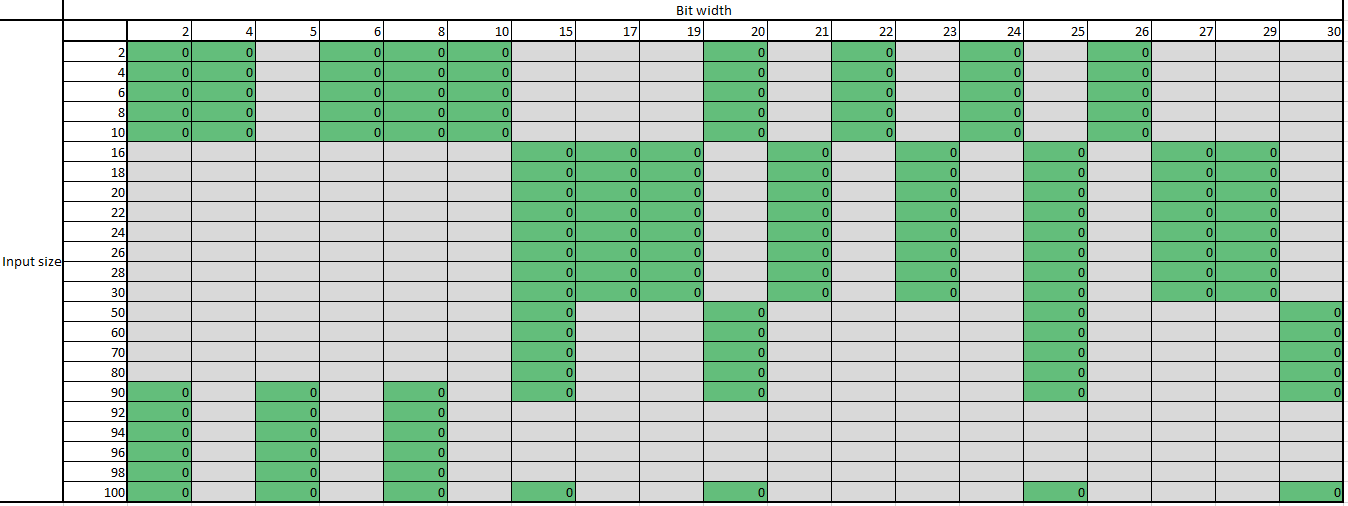
\includegraphics[width=12cm]{p4_ILP_mg.png}
\caption{Margin of error for various input size and word length combinations for ILP}
\label{fig:ilp}
\end{figure}

Each cell in the above figure is color-coded based on the margin of error
the ILP model had in its final solution. This figure is presented mostly to
contrast with the other figures in the section, as it is clear the ILP model
was able to produce an accurate solution in every instance. Comparing this result
with the same figure for the greedy algorithm below, it is abundantly clear
that the ILP approach is vastly superior in terms of accuracy. Note that the
table in Figure~\ref{fig:greedy} uses an accuracy rating that is the inverse of the
ILP table - a rating of 1 is a perfect solution and 0 is instead the worst.

\begin{figure}[h]
\centering
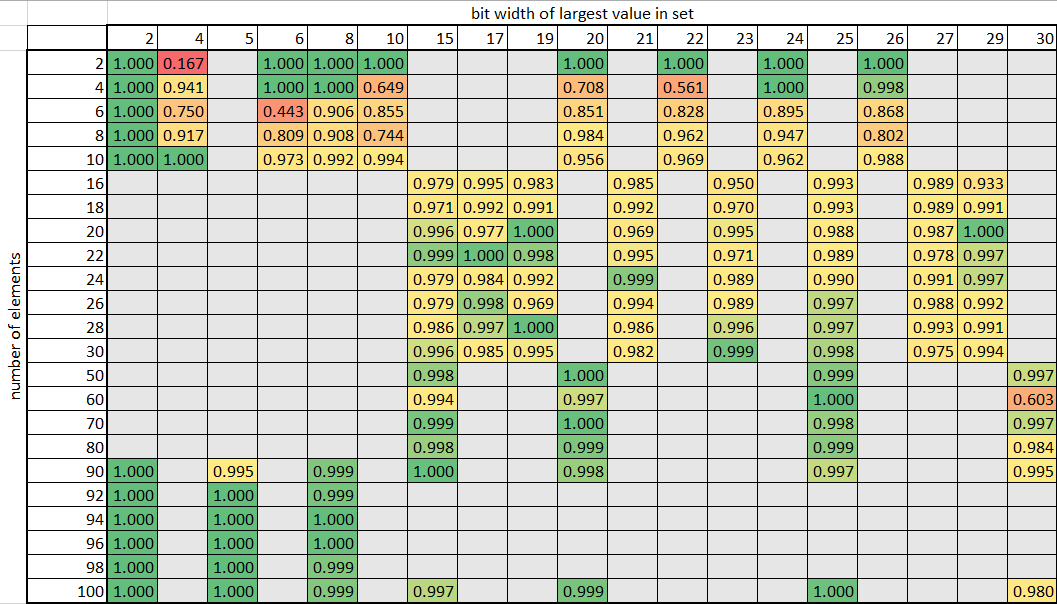
\includegraphics[width=12cm]{P3_margin.png}
\caption{Margin of error for various input size and word length combinations for the greedy algorithm}
\label{fig:greedy}
\end{figure}

Of the 151 instances that were tested, the greedy algorithm was able to
correctly solve 28 of them, yielding an 18.5\% success rate. Compared to the
ILP formulation, which had a 100\% success rate, the greedy algorithm 
is much less successful despite it's lower time complexity. As a reminder,
Figure~\ref{fig:exhaustive} shows the run-times for the exhaustive algorithm.

\begin{figure}[h]
\centering
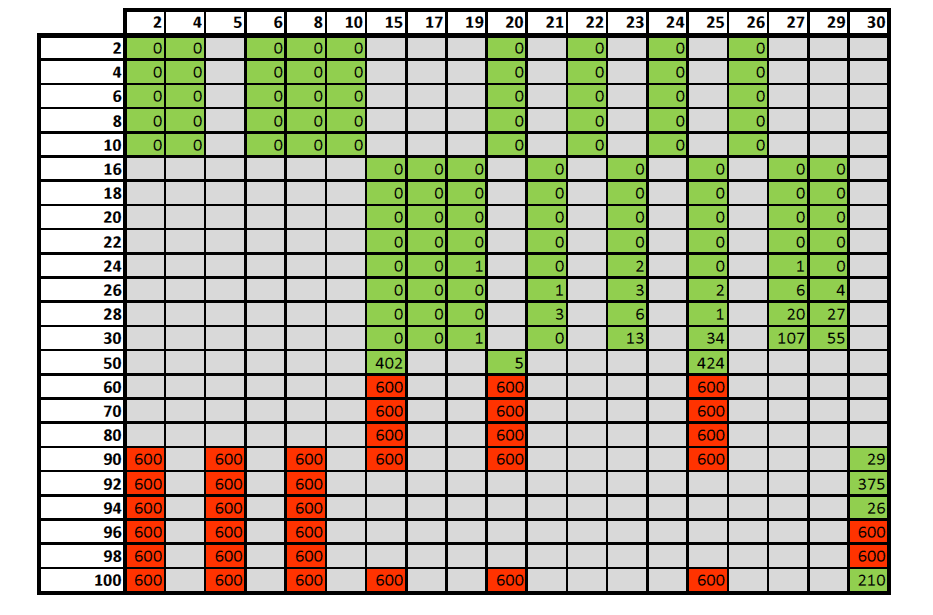
\includegraphics[width=12cm]{P1_res.png}
\caption{Run time for various input size and word length combinations for the exhaustive algorithm}
\label{fig:exhaustive}
\end{figure}

In general, the amount of margin exhibited by the greedy algorithm seems to come down to how many
subsets actually do exist within the set that satisfy the target sum, which depends on factors such 
as the distribution of integers values in the set and whether a value repeats itself.
For example, for sets with several large and small numbers that are similar to each other, there may
be more subsets that satisfy a given target sum compared to a set with a more even distribution of integers.
Granted, this also depends on the target sum itself. But if there are many subsets that satisfy the
target sum, then the greedy algorithm has a better chance of solving a given instance. 

When compared to the exhaustive algorithm, the accuracy advantage of the ILP approach is similar to
that of the greedy algorithm. However, when the timing results of the ILP algorithm in Figure~\ref{fig:ilp_rt}
are compared to that of the exhaustive algorithm, it is actually the much more primitive exhaustive
algorithm that has the advantage in solving smaller or less complex instances. This result was surprising,
as all other findings seemed to indicate that ILP was more or less a 'magic bullet' for solving our
subset sum instances.

\section{Conclusion}

Overall it seems that ILP is the best approach we have tested to date for solving subset sum instances, in
a general sense. More specifically, ILP excels at solving more complex instances that greedy or exhaustive
approaches cannot solve in a reasonable amount of time. However, due to its sophisticated approach to generating
a solution, it seems to be excessively costly for solving simpler instances. In these instances, one can reach
an optimal solution much faster by using a simpler approach. This illustrates that not only is there no perfect 
method to solve any optimization problem, but it seems that often there is no perfect method for solving every
instance of a single optimization problem.

\end{document}
